\documentclass[11pt]{article}
\usepackage[margin=1in]{geometry}
\usepackage{booktabs,graphicx,caption,subcaption,hyperref,xcolor,enumitem,amsmath,listings,float}
\hypersetup{colorlinks=true,linkcolor=black,urlcolor=blue!50!black}
\graphicspath{{../results/}{../results/dataset/}{../../results/}{../../slides/assets/}}
\setlist{itemsep=2pt}
\captionsetup{font=small}
\lstset{language=Python,basicstyle=\ttfamily\footnotesize,breaklines=true,frame=single,framerule=0.3pt,rulecolor=\color{gray!50},backgroundcolor=\color{gray!5},keywordstyle=\color{blue!60!black},commentstyle=\color{gray!70!black},stringstyle=\color{orange!70!black},showstringspaces=false,columns=fullflexible,keepspaces=true,xleftmargin=4pt,xrightmargin=4pt,aboveskip=6pt,belowskip=8pt}

\title{Teaching a Small Neural Network to Listen\\\large From counting voices in a noisy room to naming the genre of a song}
\author{Karol D\k{a}browski \\ First-Year Seminar}
\date{28 October 2026}

\begin{document}
\maketitle

\begin{abstract}
Most of the artificial intelligence we meet reads text or looks at pictures. Far less of it listens. This project asked whether the same kind of network that recognises objects in photographs could answer two questions about sound: \emph{how many people are talking?} and \emph{what kind of music is this?} The method is the same in both cases: draw the sound as a picture, a spectrogram, and let a convolutional neural network (CNN) read it.

For voices, I built a dataset of 20\,000 four-second clips by overlaying recordings of single speakers with noise and echo, and trained a CNN to count the people, and how many were male or female. It reached 80\,\% exact accuracy, and 99\,\% within one person, on speakers it had never heard. Tested on real meeting recordings it collapsed to 25\,\%, and recovered to 68\,\% after retraining on real audio.

For music, I scraped 25\,943 thirty-second previews from the Deezer API, labelled by album genre tag, across eight genres: classical, pop, jazz, hip-hop, rock, electronic, country and film score. The best CNN trained from scratch reached 77.4\,\% on songs by artists it had never heard, where chance is 12.5\,\%. A classifier with 130\,000 parameters, trained in three minutes on embeddings from a large public audio model (CLAP), reached 79.4\,\%, and the two together 79.7\,\%. On a further 504 songs from 258 new artists, collected to check that nothing had been overfitted, the ranking held and every model scored two to three points higher.

The two halves taught one lesson from two directions: with sound, the training data decides almost everything. Simulated rooms did not transfer to real rooms, and the ceiling on music genre is set by how consistently people label it, not by the size of the network.
\end{abstract}

\tableofcontents

\section{Introduction}

\subsection{Why sound?}
Ask what AI does today and the answers are mostly about words and images: chatbots, translation, face recognition, photo search. Hearing gets much less attention, even though it is one of the main ways people understand a room. Walk into a party blindfolded and you still know roughly how many people are there and what music is playing. I wanted to know whether a small network, trained on a laptop in an afternoon, could do either of those things.

Sound is also harder than it looks. In a photograph, two objects sit side by side, and a network can draw a box around each one. In audio, two voices or two instruments playing at the same time simply add together. There is one waveform, and the parts have to be pulled apart from the mixture. That is why both of my questions turned out to be about overlap: counting speakers is hard exactly when they talk over each other, and genres are hard exactly where they overlap, pop with rock, classical with film score.

\subsection{The two questions}
\begin{enumerate}
  \item \textbf{How many people are talking?} Given four seconds of audio from a noisy room, report the number of simultaneous speakers (0 to 4), and how many of them are male and female. There is no public dataset for this, so I built one, and then tested on real meetings.
  \item \textbf{What kind of music is this?} Given a thirty-second clip, name its genre out of eight. Here the data is real from the start, scraped from a public music service, and the labels come with all the ambiguity of real tags.
\end{enumerate}
A third question grew out of the second: \emph{can a model that has already heard far more music do better than one trained from scratch?} I answer it with CLAP, a public model trained on hundreds of thousands of captioned clips.

\subsection{What this report contains}
Section~\ref{sec:method} describes the data and methods for both halves, with short code excerpts where the detail matters. Section~\ref{sec:results} gives the results, including the side experiments. Section~\ref{sec:discussion} discusses what the numbers mean and what I would conclude. Section~\ref{sec:future} lists what I would do with more time. Everything was run on one laptop with an Apple M-series GPU; the longest single training run took two hours.

\section{Data and methodology}\label{sec:method}

\subsection{Sound as a picture}
Every model in this project works the same way. Audio is turned into a \emph{spectrogram}: a picture with time running left to right, pitch running bottom to top, and brightness showing how much energy there is at each pitch and moment. A voice appears as a stack of horizontal lines, its harmonics. A drum hit is a vertical stripe. A CNN, the kind of network used for images, then reads that picture like any other.

The computation has three steps. The waveform $x$ is cut into short overlapping windows and each window is Fourier-transformed, giving the short-time power spectrum $S[k,t]$ at frequency bin $k$ and frame $t$. The frequency bins are then grouped by a \emph{mel} filterbank $F$, which spaces the bands the way human hearing does, fine at low pitch and coarse at high pitch. Finally the logarithm compresses the huge range of loudness:
\[
M[m,t] = \log\Big(\sum_k F_{m,k}\,S[k,t] + 10^{-6}\Big).
\]
Figure~\ref{fig:melvsstft} shows the same clip both ways. For speech I used 64 mel bands on 16\,kHz audio over 4 seconds, giving a $64\times401$ picture. For music I used 128 bands on 22\,kHz audio over 30 seconds, giving $128\times646$.

\begin{figure}[H]\centering
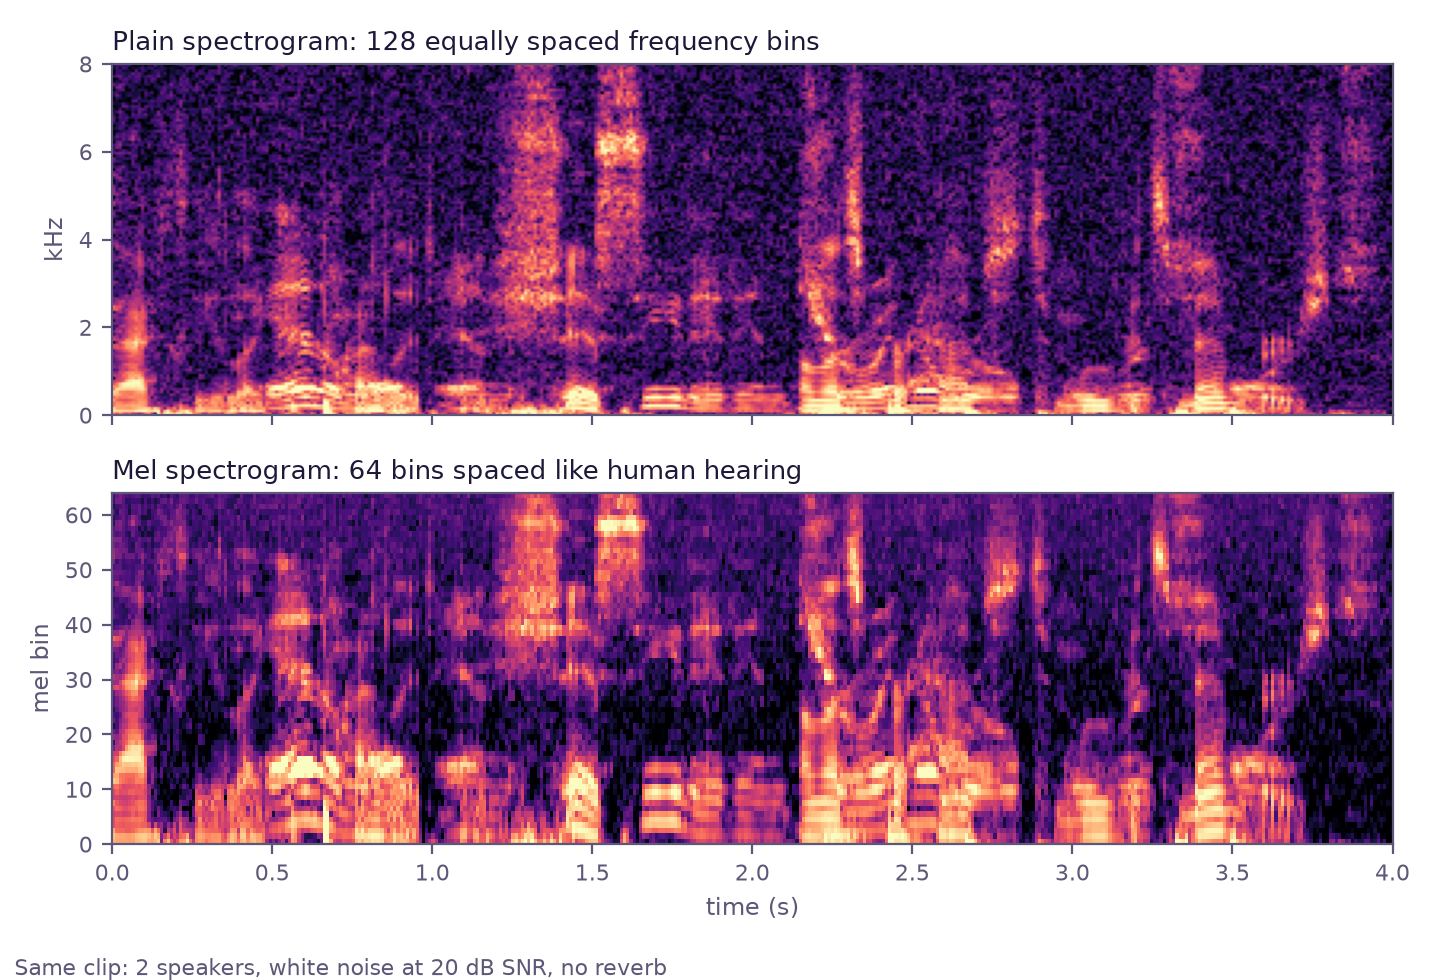
\includegraphics[width=.85\textwidth]{mel_vs_stft_light.png}
\caption{The same four-second clip (two speakers, white noise at 20\,dB) as a plain spectrogram with 128 equally spaced bins and as a mel spectrogram with 64 bins. The mel version spends its resolution where the harmonics of a voice live.}\label{fig:melvsstft}
\end{figure}

In code, the music version is four lines:
\begin{lstlisting}
_mel = torchaudio.transforms.MelSpectrogram(sample_rate=22_050, n_fft=2048, hop_length=1024,
                                            n_mels=128, f_min=20, f_max=11_025)
def log_mel(audio):                       # waveform (T,) -> (128, 646)
    return torch.log(_mel(torch.from_numpy(audio)) + 1e-6)
\end{lstlisting}

\subsection{Question 1: a voice-counting dataset I had to build}
There is no public collection of recordings labelled ``three people talking at once''. So I made one from LibriSpeech, a free set of audiobook readings in which 291 speakers (146 male, 145 female) were each recorded alone in a quiet room. The recipe for one clip:
\begin{enumerate}
  \item Pick $n$ speakers, $n$ uniform in 0 to 4, from the speakers allowed in this split.
  \item Take a random four-second excerpt from each and add them together.
  \item With probability 0.5, apply artificial reverb (echo).
  \item Pick a noise type, white, pink or ``babble'' (twelve other voices mixed together so that no single one is intelligible), and add it at a signal-to-noise ratio drawn uniformly from 0 to 20\,dB.
\end{enumerate}
Because the clip is built from known parts, the labels are exact: number of speakers, number of male, number of female, plus the noise level and type for later analysis. Speakers are split 70/15/15 into train, validation and test \emph{by speaker}, so the network never hears a test voice during training and has to count rather than recognise.
\begin{lstlisting}
def make_mixture(utts, speakers, sex, rng, max_speakers=4, snr_range=(0, 20), p_reverb=0.5):
    n_spk = rng.randint(0, max_speakers)
    chosen = rng.sample(speakers, n_spk)
    mix = sum(random_excerpt(utts[s], rng) for s in chosen)        # overlay the voices
    if rng.random() < p_reverb and n_spk > 0:
        mix = apply_reverb(mix, rng)
    noise = {"white": white, "pink": pink, "babble": babble_noise}[rng.choice(kinds)](...)
    snr_db = rng.uniform(*snr_range)
    noise *= rms(mix) / 10 ** (snr_db / 20)                          # scale noise to the SNR
    return mix + noise, dict(n_speakers=n_spk, n_male=sum(sex[s] == "M" for s in chosen), ...)
\end{lstlisting}
The final dataset (``v3'') has 20\,000 training clips, 1\,500 validation and 2\,000 test. Two further sets with the same recipe but only male or only female speakers, 20\,000 training clips each, were built for the single-sex experiment.

\subsection{Question 1, real data: the AMI Meeting Corpus}
To find out whether a model trained on built clips survives real rooms, I used the AMI Meeting Corpus: about 100 hours of real four-person meetings recorded with a microphone array on the table and headsets, with time-stamped speaker turns and the sex of every participant. Cutting the recordings into four-second windows with a two-second hop, and counting a speaker if they talk for at least half a second in the window, gives exact labels for free. I used 136 meetings for training (42\,510 windows, balanced across counts) and held-out meetings for testing (8\,000 windows at their natural distribution, in which one speaker dominates, plus a balanced set of 1\,689).

\subsection{Question 2: scraping music from Deezer}
Spotify no longer serves audio previews through its API, so the music data comes from Deezer's public API, which returns a thirty-second MP3 for almost any track with no key. The crawler works genre by genre:
\begin{enumerate}
  \item \textbf{Seeds.} Start from Deezer's own chart, editorial playlists and radios for that genre, and collect the artists in them.
  \item \textbf{Expansion.} Walk breadth-first over Deezer's ``related artists'' links.
  \item \textbf{Purity filter.} Fetch each artist's albums. Keep the artist only if at least half of their albums carry the target genre tag. This removes artists who merely appear on a genre playlist.
  \item \textbf{Labels.} A track's label is its album's genre tag, which must equal the target genre.
  \item \textbf{Caps.} At most four tracks per album and twelve per artist, so no artist dominates. An artist may appear in only one genre; any artist found under two genres is dropped entirely.
\end{enumerate}
\begin{lstlisting}
albums = get_all(f"/artist/{aid}/albums", max_items=100)
hits   = [a for a in albums if a.get("genre_id") == gid]        # albums tagged with this genre
purity = len(hits) / len(albums)
if purity < 0.5 or len(hits) == 0:
    continue                                                       # not really a <genre> artist
for alb in hits[:12]:                                              # then take up to 4 tracks per album
    for t in random.sample(album_tracks(alb), 4): ...
\end{lstlisting}
Film score needed special handling. Deezer's ``Films/Games'' tag is full of pop songs that appear in movies, so for that class I skipped the charts and seeded from 65 film and game composers (Zimmer, Williams, Morricone, G\"oransson, Gu\dh nad\'ottir, Hisaishi and so on) plus the ``Epic Soundtracks'' and ``Film Scores'' playlists, and let the related-artist walk expand from there.

Two practical lessons cost about an hour each. Preview links carry a signed token that expires within minutes, so a link gathered at the start of a crawl is dead by the time the download loop reaches it; the fix is to download immediately or re-fetch the link. And after roughly ten thousand fast downloads the preview server starts answering ``429 Too Many Requests''; a slow, single-threaded retry with a thirty-second back-off recovers the rest.

\paragraph{Splits.} The split is by \emph{artist}, 80/10/10, stratified per genre. This is the music equivalent of unseen speakers: every test song is by an artist the model never heard, so it must recognise genres, not artists. A song-level split would let the network recognise a singer's voice or an album's production and report a flattering number.
\paragraph{Two crawls.} The first crawl gave 12\,699 clips from about 1\,100 artists. A second crawl, run later to test whether more data helps, added 13\,244 clips from new artists only, bringing the total to 25\,943. The validation and test clips were frozen before the second crawl, so every model in this report is scored on exactly the same test songs.
\paragraph{Fresh set.} Finally, to be sure no number was a lucky split, I scraped 504 more clips, 63 per genre, from 258 artists that appear nowhere in training, validation or test, and scored every model on them as well.

\begin{figure}[H]\centering
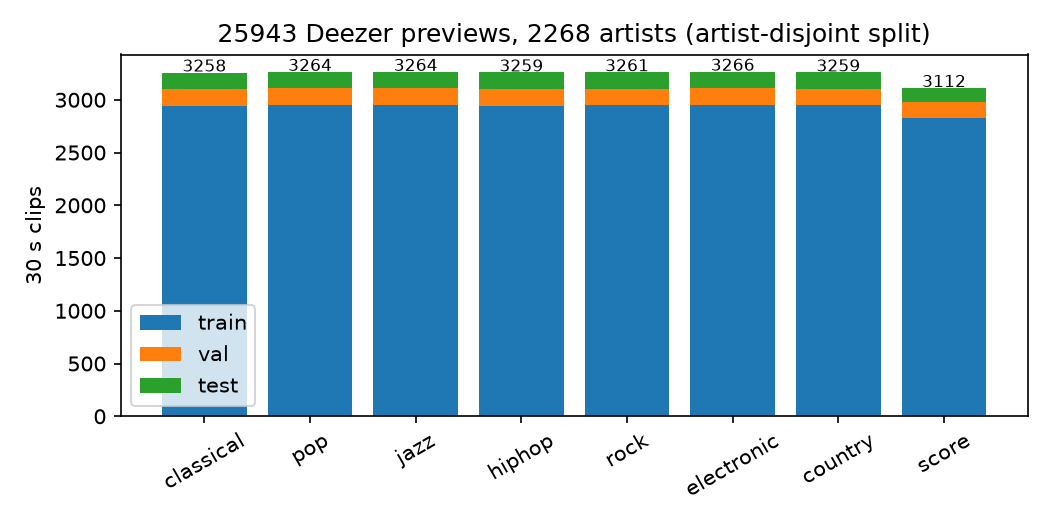
\includegraphics[width=.75\textwidth]{class_counts.png}
\caption{The music dataset after the second crawl: about 3\,250 clips per genre, split by artist. Validation and test are unchanged from the first crawl.}
\end{figure}
\begin{figure}[H]\centering
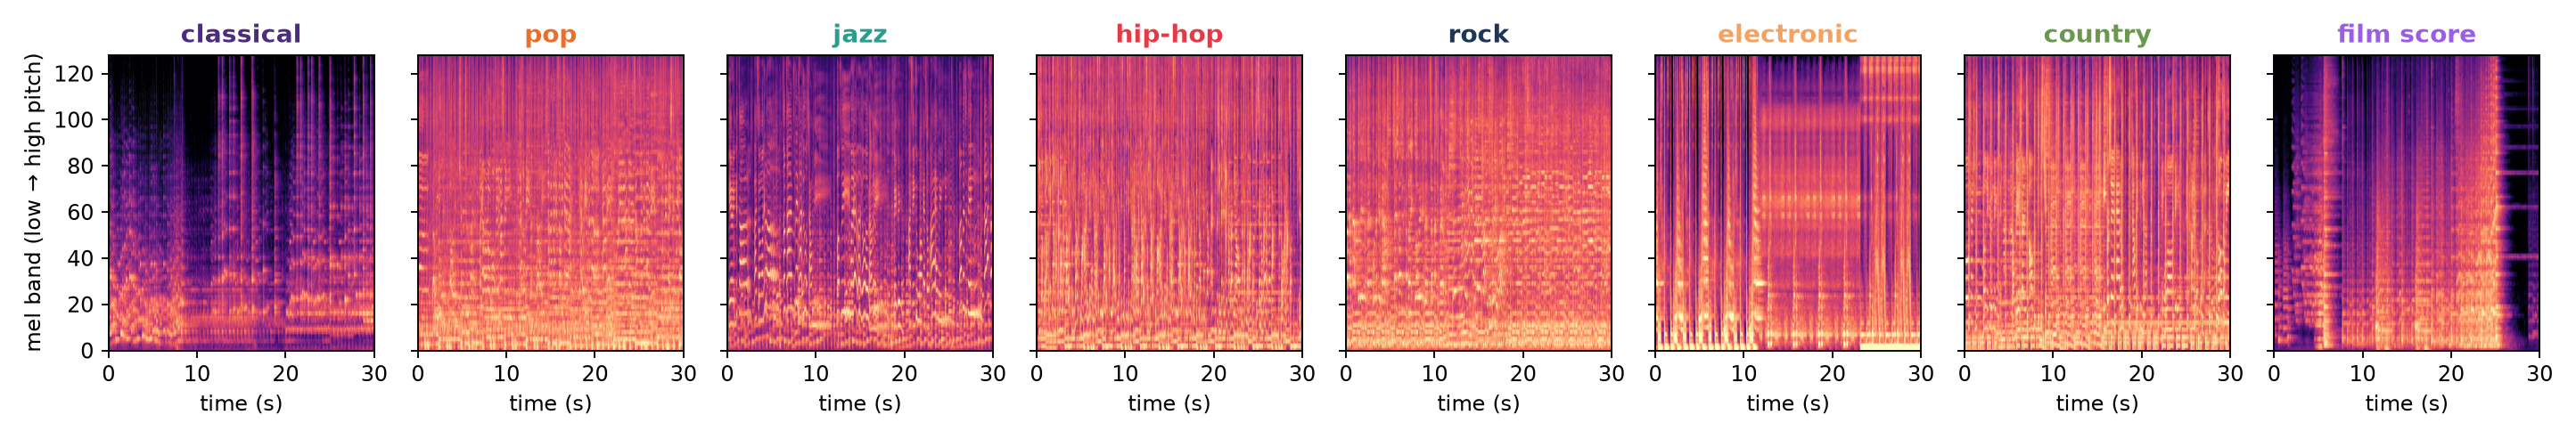
\includegraphics[width=\textwidth]{typical_spectrograms.png}
\caption{One typical clip per genre, chosen as the clip closest to its genre's average spectrum, on a shared colour scale. Classical and film score are sparse and quiet; pop, rock and hip-hop are dense walls of sound; electronic has hard-edged blocks and a steady beat.}
\end{figure}
\begin{figure}[H]\centering
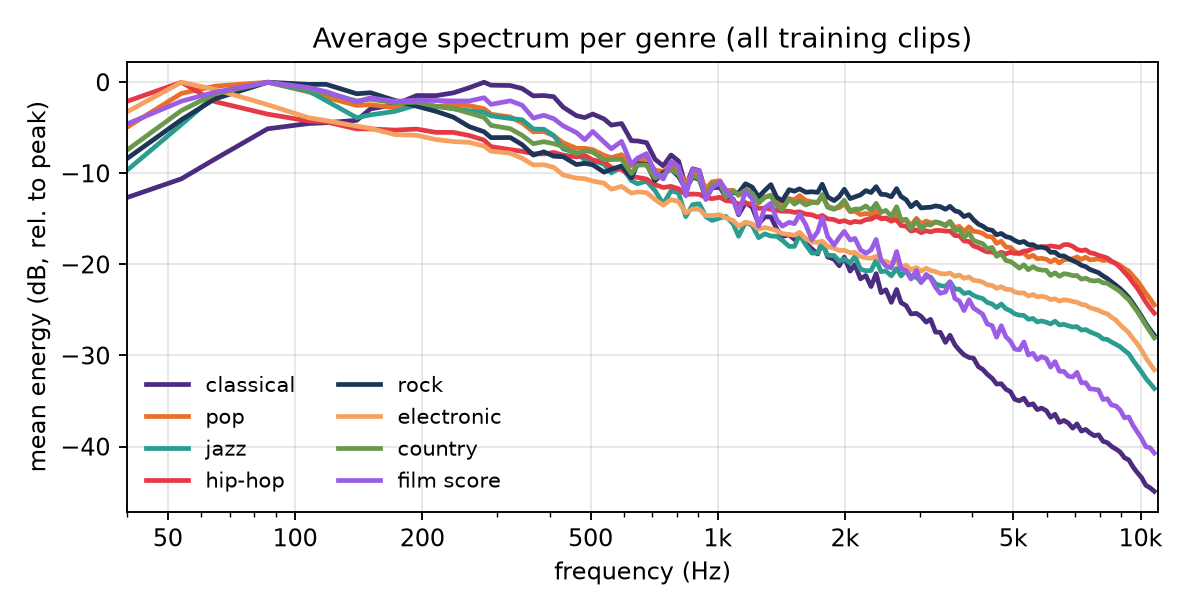
\includegraphics[width=.72\textwidth]{mean_spectrum.png}
\caption{Average spectrum of all training clips in each genre, relative to each genre's own peak. Classical and film score have almost no energy above 2\,kHz; rock and hip-hop have the most. This is the kind of regularity a network can use, but it is nowhere near enough on its own.}
\end{figure}

\subsection{The networks}
Both halves use the same family of network, a small VGG-style CNN: a stack of blocks, each with two $3{\times}3$ convolutions, batch normalisation and a ReLU, followed by a max-pool that halves the picture. After the blocks, global pooling collapses whatever is left into one vector regardless of clip length, and a small fully connected head produces the answer.

\paragraph{Voice counter.} Four blocks with 32, 64, 128 and 128 filters, global average pooling to 128 numbers, and \emph{three} output heads, each a five-way classifier (0 to 4): total speakers, male speakers, female speakers. The loss is the sum of the three cross-entropies. About 0.6 million parameters.
\begin{lstlisting}
self.heads = nn.ModuleDict({k: nn.Linear(width * 4, 5) for k in ["n_speakers", "n_male", "n_female"]})
def forward(self, x):
    h = self.pool(self.features(self.norm(x))).flatten(1)
    return {k: head(self.dropout(h)) for k, head in self.heads.items()}
\end{lstlisting}

\paragraph{Genre classifier.} Five blocks with widths $w, 2w, 4w, 8w, 8w$, global average \emph{and} max pooling concatenated, then dropout, a 256-unit layer, dropout, and the eight-way output. With $w=32$ this is 2.49 million parameters (cnn\_v1 to v3); with $w=48$ it is 5.49 million (cnn\_v4).
\begin{lstlisting}
class GenreCNN(nn.Module):
    def __init__(self, n_classes=8, width=32, p=0.3):
        super().__init__()
        self.norm = nn.BatchNorm2d(1)
        self.features = nn.Sequential(conv_block(1, width), conv_block(width, 2*width),
            conv_block(2*width, 4*width), conv_block(4*width, 8*width), conv_block(8*width, 8*width))
        self.head = nn.Sequential(nn.Dropout(p), nn.Linear(16*width, 256), nn.ReLU(), nn.Dropout(p),
                                  nn.Linear(256, n_classes))
    def forward(self, x):
        h = self.features(self.norm(x))
        h = torch.cat([h.mean((2, 3)), h.amax((2, 3))], 1)     # global average + max pooling
        return self.head(h)
\end{lstlisting}

\subsection{Training}
\paragraph{Voices.} AdamW with learning rate $5\times10^{-4}$, batch 64, 30 passes over the training clips, an exponential moving average of the weights, and light SpecAugment (one random frequency band and one random time span masked per clip). The checkpoint with the best validation accuracy is kept. About 1.5 hours per model.

\paragraph{Music.} AdamW with learning rate $10^{-3}$ and weight decay $10^{-2}$, a one-cycle learning-rate schedule, batch 64, cross-entropy with label smoothing $\epsilon=0.1$ and class weights proportional to $(N/n_c)^{1/2}$ to even out small imbalances. The network trains on random \emph{ten-second} crops of the thirty-second spectrogram with SpecAugment (two frequency masks, two time masks) and a random gain; this acts like having many more clips. At test time it sees the full thirty seconds, which the global pooling allows.
\begin{lstlisting}
def __getitem__(self, i):                       # training view of one clip
    x = self.x[i].float()
    t0 = np.random.randint(0, x.shape[1] - 216 + 1)
    x = x[:, t0:t0 + 216]                        # random 10 s crop
    for _ in range(2):                           # SpecAugment: 2 frequency + 2 time masks
        f = np.random.randint(0, 16); f0 = np.random.randint(0, 128 - f); x[f0:f0 + f] = x.mean()
        t = np.random.randint(0, 21); t0 = np.random.randint(0, 216 - t); x[:, t0:t0 + t] = x.mean()
    return (x + 0.1 * np.random.randn()).unsqueeze(0), self.y[i]
\end{lstlisting}
The models, in the order they were trained: cnn\_v1 (seven genres, 30 epochs, classical under-represented because of the download throttling), cnn\_v2 (seven genres, full data, 40 epochs), cnn\_v3 (cnn\_v2's weights with a new eight-way head, fine-tuned 9 epochs after film score was added), and cnn\_v4 ($w=48$, trained from scratch for 11 epochs on the doubled data).

\begin{figure}[H]\centering
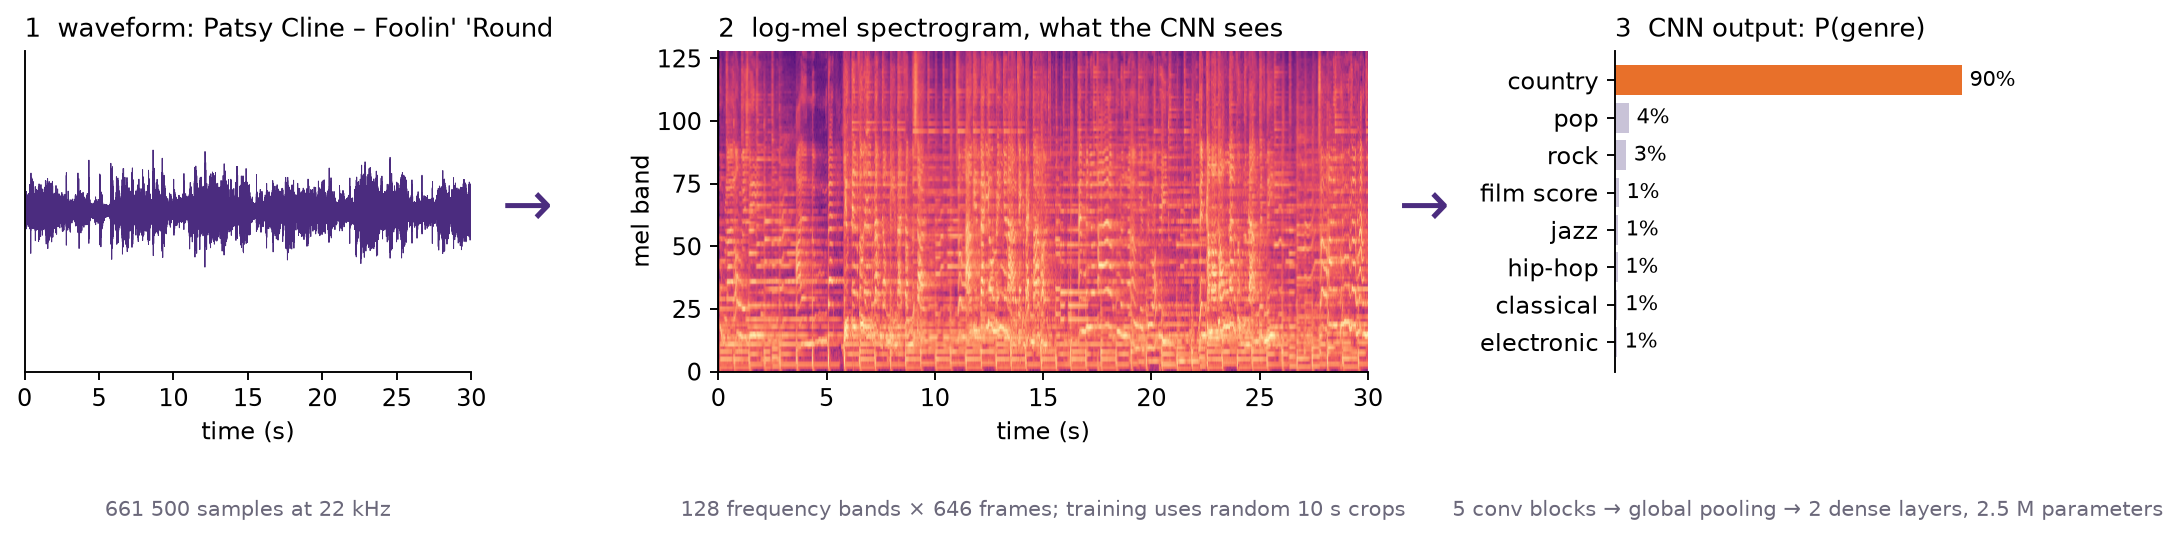
\includegraphics[width=\textwidth]{pipeline_example.png}
\caption{One test clip through the genre pipeline: the waveform, its log-mel spectrogram, and the network's output, here Patsy Cline recognised as country with 90\,\%.}
\end{figure}

\subsection{CLAP: borrowing ears}\label{sec:clapmethod}
My networks learned what music sounds like from scratch, from a few thousand clips. CLAP (Contrastive Language-Audio Pretraining, released by LAION) learned from hundreds of thousands of audio clips paired with text captions. It has two encoders: one turns any clip into a vector of 512 numbers, an \emph{embedding}, and the other turns any sentence into a vector of 512 numbers. Training pushed matching pairs together and non-matching pairs apart, so ``a jazz trumpet solo'' and a recording of one end up as nearby vectors. The audio encoder is a transformer with about 80 million parameters that itself reads a mel spectrogram. I used the \texttt{laion/larger\_clap\_general} checkpoint; the music-specific checkpoint loads with a broken temperature under the current library version and could not be used.

\paragraph{Zero-shot.} No training at all. Embed the clip as $\mathbf{a}$, embed a few sentences per genre and average them into $\mathbf{t}_c$ (two descriptions such as ``country music'' and ``a country song'', each in three templates such as ``This is \{\}.''), then
\[
p_c = \operatorname{softmax}_c\big(\tau \cos(\mathbf{a},\mathbf{t}_c)\big), \qquad \tau = e^{\text{logit\_scale}}\approx 39 .
\]
The temperature $\tau$ is a number CLAP learned; it is why zero-shot probabilities look extremely confident. CLAP's native input is ten seconds, so a thirty-second clip is embedded as three chunks whose vectors are averaged.
\begin{lstlisting}
def probs(audio_22k):
    a = resample(audio_22k, 22_050, 48_000)
    chunks = [a[i:i + 480_000] for i in range(0, len(a) - 480_000 + 1, 480_000)]   # 10 s each
    ae = normalize(model.get_audio_features(**proc(audio=chunks, sampling_rate=48_000)))
    ae = normalize(ae.mean(0, keepdim=True))
    logits = model.logit_scale_a.exp() * ae @ T.T        # T: 8 averaged text embeddings
    return logits.softmax(-1)[0]
\end{lstlisting}

\paragraph{Embeddings plus a small classifier.} Embed each of my clips once (about 30 minutes for 12\,699 clips), then train a tiny network on those 512-number vectors with my labels: 512 inputs, one hidden layer of 256 with GELU, 8 outputs, 130\,000 parameters, dropout 0.5, weight decay 0.1, 300 epochs with a cosine schedule. The hidden size, dropout and weight decay were chosen on the validation split from a grid of twelve settings. CLAP itself stays frozen. Training took three minutes. This is standard \emph{transfer learning}: the big model supplies the ears, the small one learns where my genre boundaries fall.

\paragraph{Ensemble.} The mean of the cnn\_v4 and CLAP-classifier probabilities.

\subsection{Evaluation}
\begin{itemize}
  \item \textbf{Voices.} Exact accuracy and ``within one'' accuracy for each head, broken down by true count, noise type, SNR band and reverb. The main test set is 2\,000 clips from unseen speakers; the real-data test set is 8\,000 AMI windows from unseen meetings.
  \item \textbf{Music.} Accuracy and macro-F1 (the mean of per-genre F1 scores, so each genre counts equally) on the frozen test split (1\,204 clips, 8 genres) and on the fresh set (504 clips). Chance is 12.5\,\%. Confusion matrices are row-normalised: each row is a true genre and sums to one.
  \item \textbf{Clip length.} Accuracy as a function of how much of the clip the network is allowed to hear, using centre crops of 2 to 30 seconds.
  \item \textbf{Humans.} I took the voice-counting test myself on 40 clips, and listened to a handful of real meeting windows, as a sanity check on how hard the task is.
\end{itemize}

\section{Results}\label{sec:results}

\subsection{Counting voices on built clips}
\begin{table}[H]\centering\small
\begin{tabular}{lcccc}\toprule
model & training clips & test clips & exact speaker count & within one \\\midrule
cnn\_v1 (first attempt) & 4\,000 & 500 & 68\,\% & 90\,\% \\
cnn\_v2 & 20\,000 & 1\,000 & 80\,\% & 98\,\% \\
cnn\_v3 (regularised) & 20\,000 & 1\,000 & 79\,\% & 98\,\% \\
cnn\_v4 (final recipe, v3 data) & 20\,000 & 2\,000 & \textbf{80\,\%} & \textbf{99\,\%} \\\bottomrule
\end{tabular}
\caption{Voice counting on synthetic clips from unseen speakers. Male and female counts for cnn\_v4: 75\,\% and 78\,\% exact, both 99\,\% within one.}
\end{table}
Going from 4\,000 to 20\,000 training clips was worth twelve points; nothing I changed in the network afterwards was worth more than one. Figure~\ref{fig:v4summary} shows where the final model fails. Silence and one speaker are nearly perfect. Two speakers reach 72\,\%, four reach 78\,\%, and three is the hard case at 56\,\%: three voices are heard as four (123 clips) more often than as two (44). The confusion is almost entirely between neighbouring counts; being off by two or more is rare. Accuracy falls with noise, from 76\,\% at 15 to 20\,dB to 70\,\% at 0 to 5\,dB, and babble noise (72\,\%) is worse than pink (84\,\%) or white (83\,\%), because babble is itself made of voices. Reverb costs thirteen points (85\,\% dry, 72\,\% with echo).
\begin{figure}[H]\centering
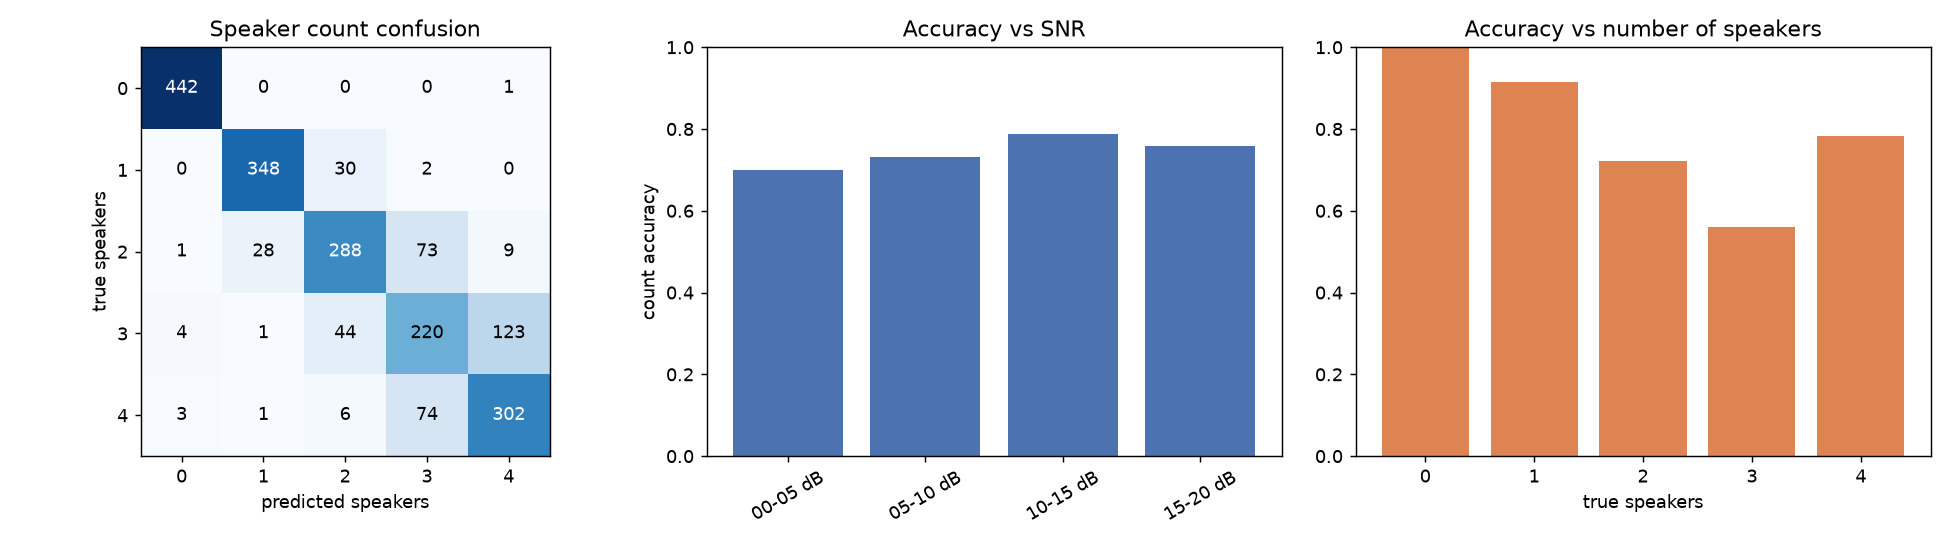
\includegraphics[width=\textwidth]{cnn_v4/summary.png}
\caption{cnn\_v4 on 2\,000 synthetic test clips: confusion matrix of the speaker count, accuracy by signal-to-noise ratio, and accuracy by true count.}\label{fig:v4summary}
\end{figure}

\subsection{Side experiment: mel vs.\ plain spectrogram}
Everything identical, same clips, network, schedule and random seed, except the input: 64 mel bands or 128 equally spaced bins. The mel model scored 83.4\,\% on one test set and the plain model 81.4\,\%; on the main test set 80.0 against 79.3\,\%. Mel also trained twice as fast because its input is half the size. One run each, so the gap is suggestive rather than proven, but there was no reason to switch away from mel.

\subsection{Side experiment: single-sex voices}
Is counting easier when every voice in the clip is the same sex? Two new synthetic sets, one from the 146 male speakers only, one from the 145 female speakers only, same recipe, and two specialist models trained on them.
\begin{table}[H]\centering\small
\begin{tabular}{lccc}\toprule
 & male-only test & female-only test & mixed test \\\midrule
mixed model (cnn\_v4) & 79.9\,\% & 76.5\,\% & 80.0\,\% \\
male-only model & \textbf{82.2\,\%} & 74.6\,\% & 79.9\,\% \\
female-only model & 70.5\,\% & \textbf{78.7\,\%} & 77.3\,\% \\\bottomrule
\end{tabular}
\caption{Exact speaker-count accuracy, 2\,000 clips per test set.}
\end{table}
Specialists win on their own sex by about two points and lose five to nine on the other, so one mixed model is the safer choice. Female voices were harder for every model. Figure~\ref{fig:sex} shows why: female harmonics are spaced roughly twice as far apart, so when two or three female voices overlap their harmonics interleave and blur into one another more easily. A caveat: the single-sex splits were drawn separately, so a few test speakers overlap with the mixed model's training set, which if anything flatters the mixed model.
\begin{figure}[H]\centering
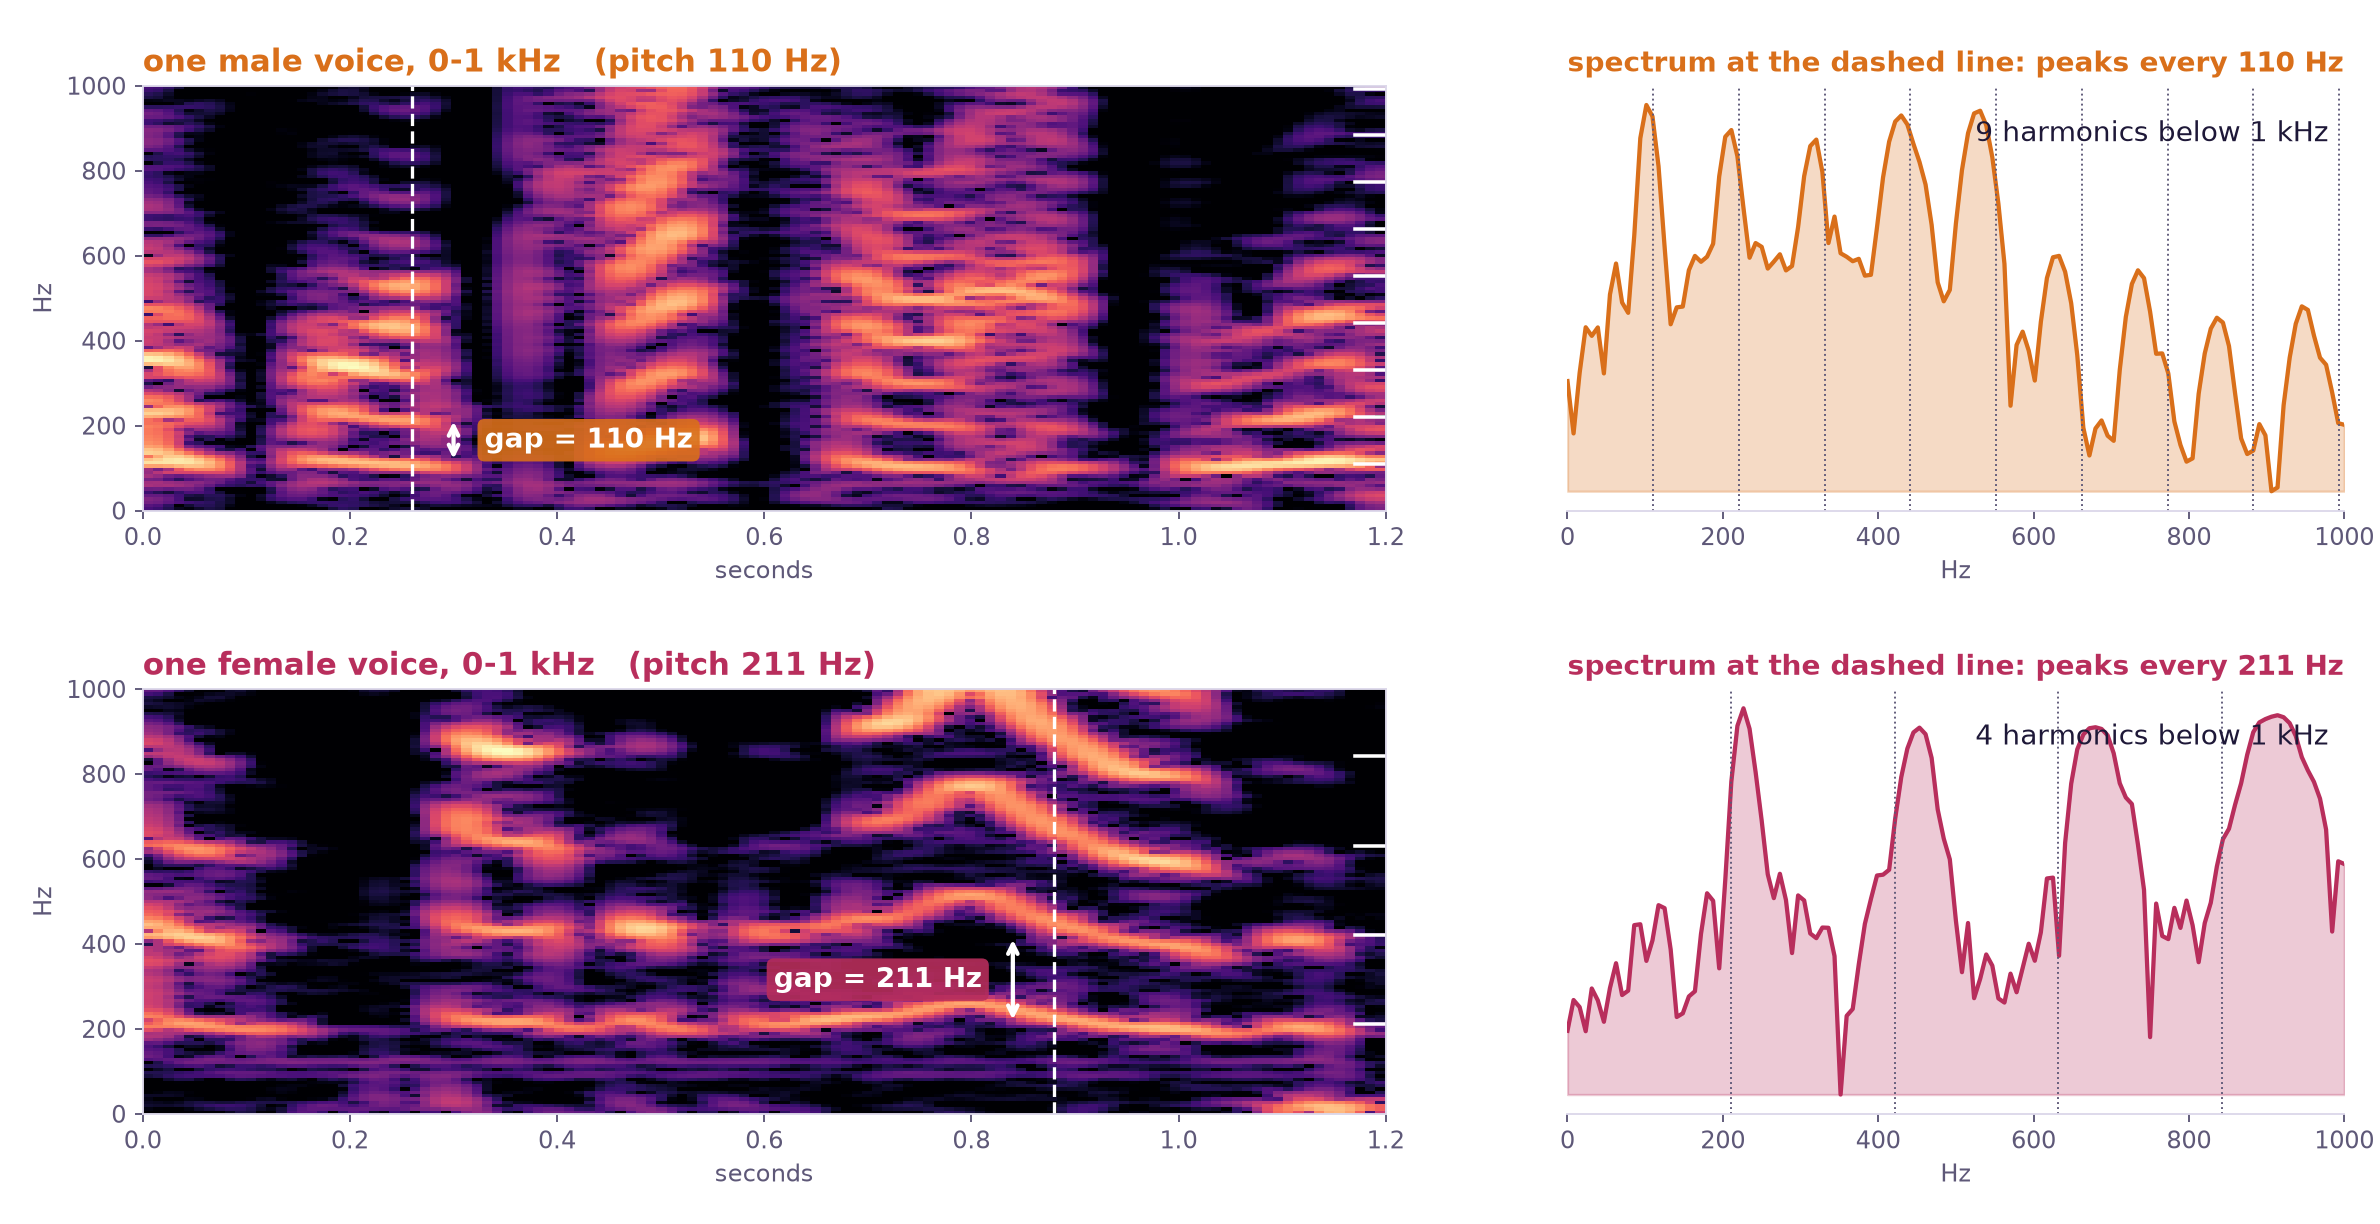
\includegraphics[width=.8\textwidth]{male_vs_female_light.png}
\caption{One male voice (pitch 110\,Hz) and one female voice (211\,Hz), as spectrogram and as the spectrum at one instant.}\label{fig:sex}
\end{figure}

\subsection{A human check}
I took the test myself on 40 synthetic clips and scored 45\,\% exact, against the model's 75\,\% on the same 40. Counting overlapping voices is hard for people too, and the model's 80\,\% is well above an untrained listener.

\subsection{Real meetings: collapse and recovery}
\begin{table}[H]\centering\small
\begin{tabular}{lcc}\toprule
model & exact count & within one \\\midrule
cnn\_v4, trained on synthetic clips only & 25\,\% & 78\,\% \\
cnn\_v6, retrained from scratch on 42\,510 real windows & \textbf{68\,\%} & \textbf{97\,\%} \\
cnn\_v7, fine-tuned from cnn\_v4 on the same windows & 66\,\% & 97\,\% \\
always answer ``one speaker'' & 60\,\% & -- \\\bottomrule
\end{tabular}
\caption{8\,000 real AMI test windows from meetings not used in training.}
\end{table}
\begin{figure}[H]\centering
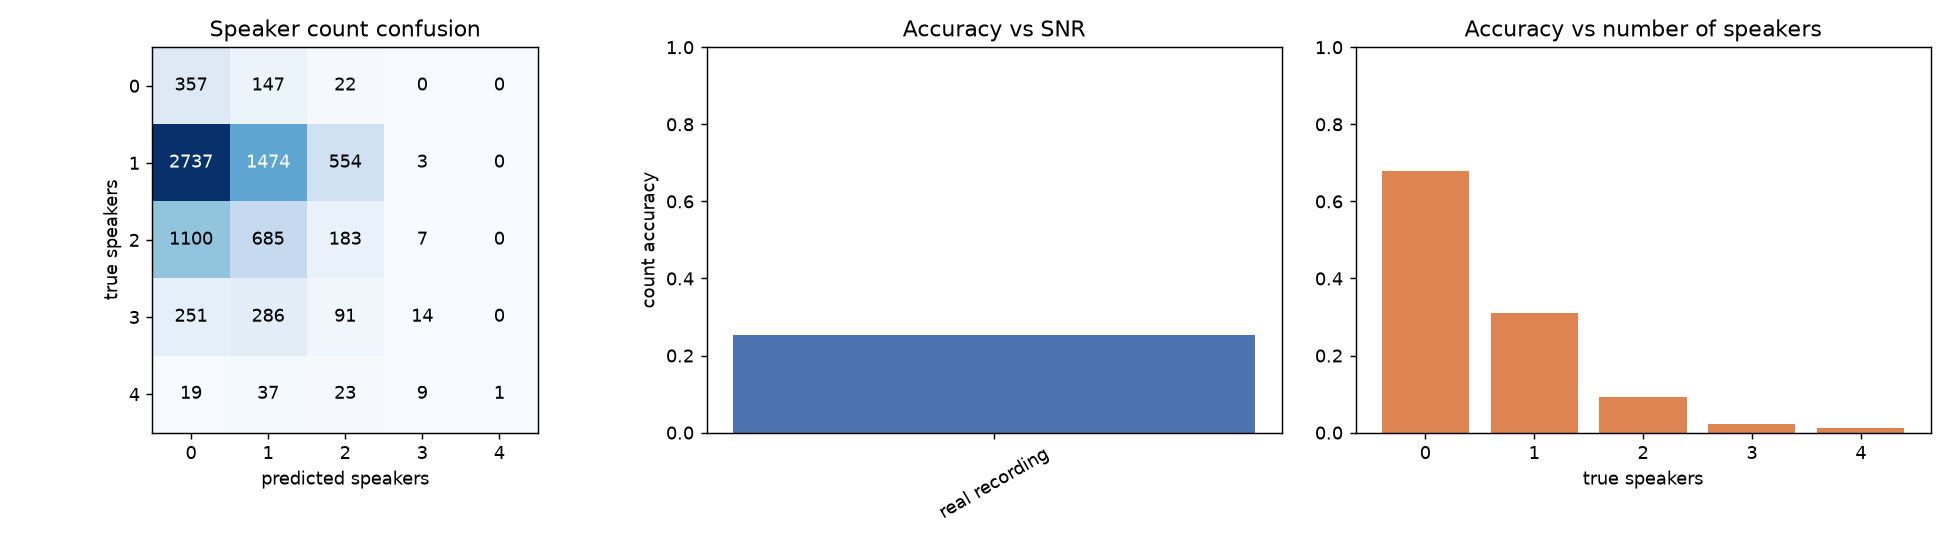
\includegraphics[width=\textwidth]{cnn_v4_on_ami_test/summary.png}
\caption{The synthetic-only model on real meetings. Most windows are called ``0 speakers'': far-field room audio is quieter and more echoey than anything in the training clips.}
\end{figure}
\begin{figure}[H]\centering
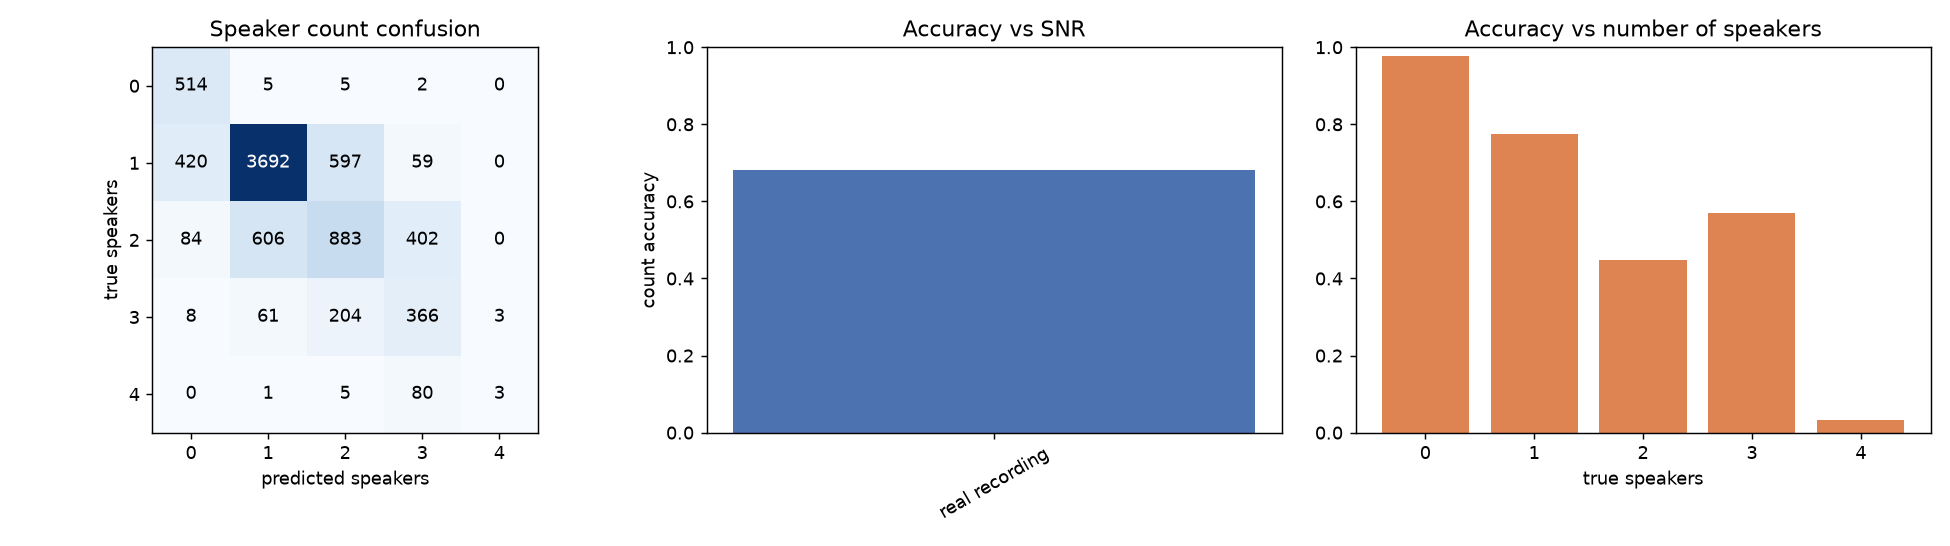
\includegraphics[width=\textwidth]{cnn_v6_ami_on_ami_test/summary.png}
\caption{The model retrained on real meetings. One speaker is now 77\,\%, but two overlapping speakers reach only 45\,\%, and four speakers (89 windows) are almost always counted as three.}
\end{figure}
The 80\,\% model fell to 25\,\%, worse than always guessing ``one''. It labelled most real speech as silence, because the table microphone's quiet, reverberant sound was outside anything it had heard. Retraining on real meetings fixed that: 68\,\% exact, 97\,\% within one. Two overlapping speakers stayed hard (45\,\%): real overlaps are brief interjections, and the window mostly sounds like one person. Four speakers at once almost never happens in a real meeting (89 windows out of 8\,000), and those are counted as three. The fine-tuned model did no better than training from scratch, and it forgot the synthetic task, dropping from 80 to 38\,\% there.

\subsection{Music genre: the CNNs}
\begin{table}[H]\centering\small
\begin{tabular}{lcccc}\toprule
model & genres & training clips & test accuracy & macro F1 \\\midrule
cnn\_v1 (30 epochs, classical short) & 7 & 8\,208 & 78.3\,\% & 0.79 \\
cnn\_v2 (40 epochs) & 7 & 9\,038 & 79.2\,\% & 0.79 \\
cnn\_v3 (adds film score, fine-tuned from cnn\_v2) & 8 & 10\,214 & 75.4\,\% & 0.75 \\
cnn\_v4 ($w=48$, from scratch, doubled data) & 8 & 23\,458 & \textbf{77.4\,\%} & \textbf{0.77} \\\bottomrule
\end{tabular}
\caption{Genre CNNs on their test splits (981 to 1\,068 clips for seven genres, 1\,204 for eight). Chance is 14.3\,\% for seven genres and 12.5\,\% for eight. cnn\_v1's split was redrawn afterwards, so its number is on an earlier split.}
\end{table}
\begin{figure}[H]\centering
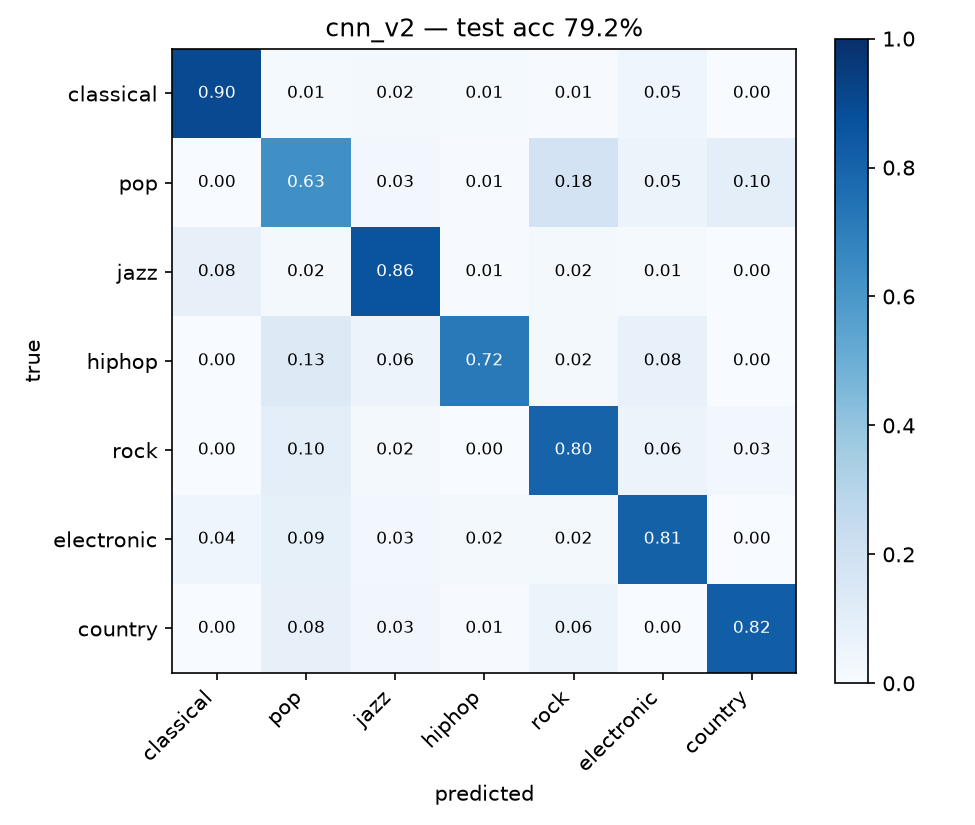
\includegraphics[width=.49\textwidth]{cnn_v2/confusion_test.png}\hfill
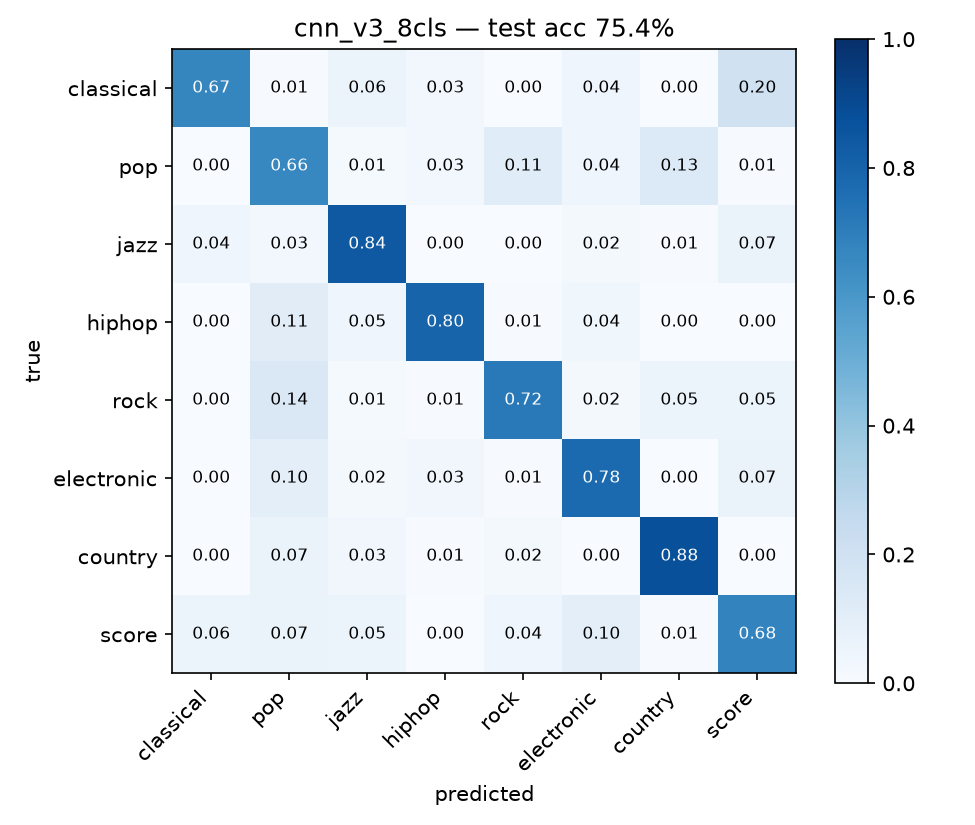
\includegraphics[width=.49\textwidth]{cnn_v3_8cls/confusion_test.png}
\caption{Left: the seven-genre model. Right: the same network after film score was added. Classical recall drops from 0.90 to 0.67; one in five classical clips is now called a film score.}
\end{figure}
\begin{figure}[H]\centering
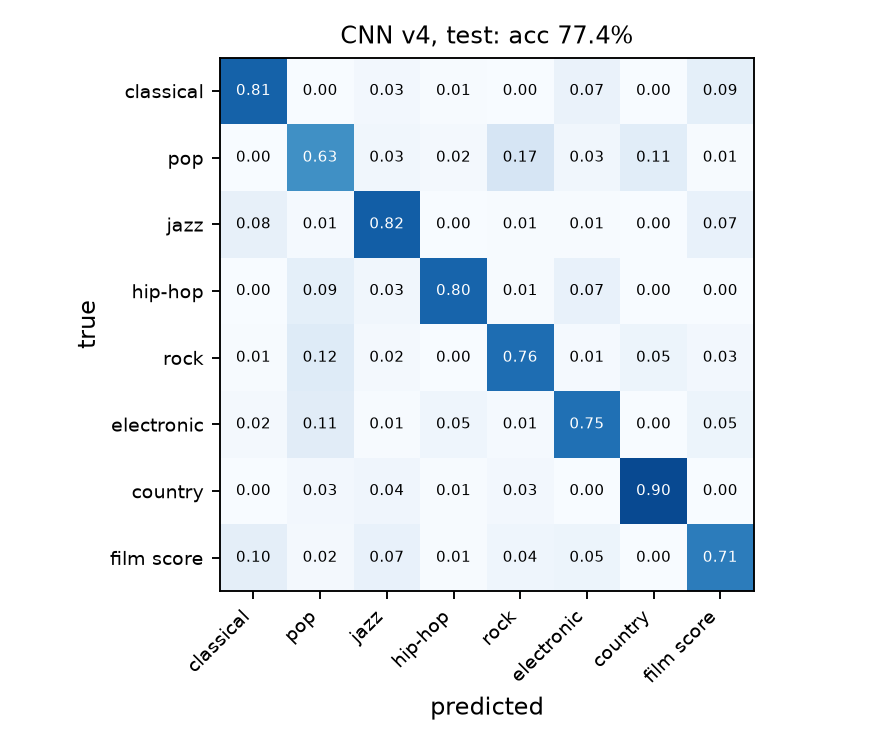
\includegraphics[width=.49\textwidth]{confusion_cnn_v4_w48_test.png}\hfill
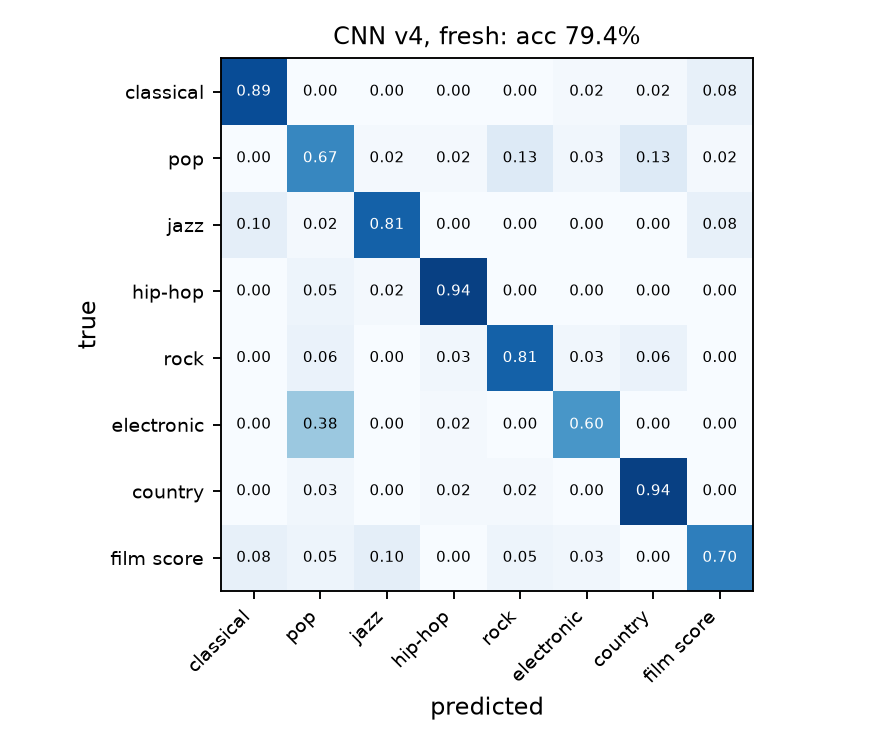
\includegraphics[width=.49\textwidth]{confusion_cnn_v4_w48_fresh.png}
\caption{cnn\_v4 on the test split (left) and on the fresh 504 songs (right). The pattern is the same on both: pop leaks into rock and country, classical and film score trade places.}
\end{figure}
\begin{figure}[H]\centering
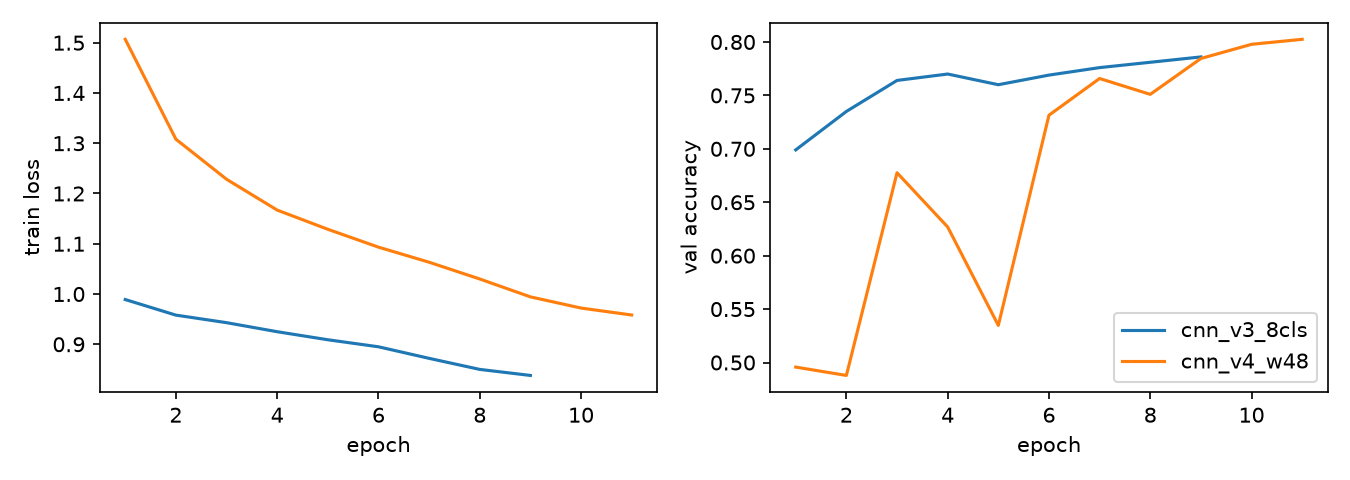
\includegraphics[width=.6\textwidth]{curves_cnn_v3_8cls_cnn_v4_w48.png}
\caption{Training curves. cnn\_v3 is shown for its nine fine-tuning epochs; cnn\_v4 for its eleven epochs from scratch. cnn\_v4's validation accuracy was still rising when training stopped.}
\end{figure}

\subsection{Where the genre models go wrong}
Two kinds of mistake dominate, and no model in the project got rid of them.
\begin{itemize}
  \item \textbf{Pop is a catch-all.} For cnn\_v4, 11\,\% of pop songs are called rock and 13\,\% country, and rock, hip-hop and electronic each leak 10 to 14\,\% into pop. Pop has the lowest F1 of any genre in every model, 0.59 to 0.69. This is the labels, not the network: Deezer tags whole albums, and ``pop'' covers everything from Carole King to Dua Lipa.
  \item \textbf{Classical and film score sound alike.} Adding film score cost classical recall, from 0.90 to 0.67. One in five classical clips is called a score, and scores drift to classical and electronic. Same orchestra, different production. Recordings of classical pieces with modern, close-miked production, such as a ``relaxing Vivaldi'' compilation, are called film score with high confidence.
\end{itemize}
The remaining genres are comfortable: hip-hop, country, jazz and classical all sit at F1 0.80 to 0.93 in the final models.

\subsection{How much audio does the network need?}
\begin{table}[H]\centering\small
\begin{tabular}{lcccccc}\toprule
clip length & 2\,s & 3\,s & 5\,s & 10\,s & 15\,s & 30\,s \\\midrule
cnn\_v2 (7 genres) & 60.9 & 68.8 & 73.2 & 76.0 & 77.8 & 79.3 \\
cnn\_v3 (8 genres) & 52.0 & 62.2 & 67.4 & 75.0 & 73.5 & 75.6 \\\bottomrule
\end{tabular}
\caption{Test accuracy (\%) as a function of the centre-cropped clip length. The models were trained on ten-second crops.}
\end{table}
\begin{figure}[H]\centering
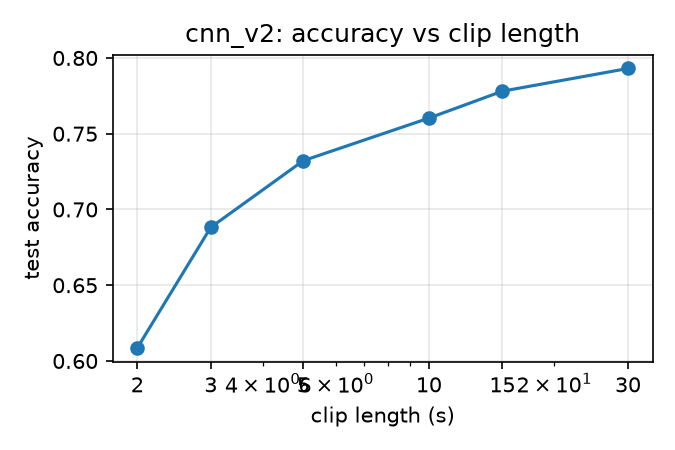
\includegraphics[width=.45\textwidth]{cnn_v2/acc_vs_cliplen.png}\hfill
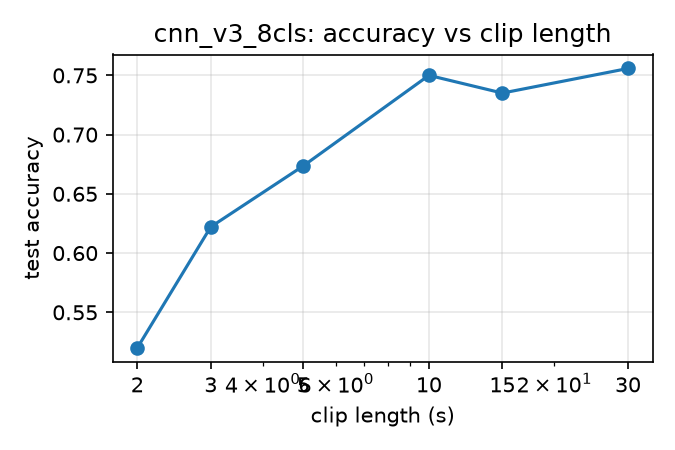
\includegraphics[width=.45\textwidth]{cnn_v3_8cls/acc_vs_cliplen.png}
\caption{Accuracy against clip length for the seven-genre and eight-genre CNNs.}
\end{figure}
Two seconds is enough to beat chance by a wide margin, ten seconds gets most of the way, and the full thirty seconds adds a few more points. In the demo this is visible as the per-window guess changing across a song, most often during intros and quiet passages.

\subsection{Music genre: CLAP}
\begin{table}[H]\centering\small
\begin{tabular}{lrcccc}\toprule
 & trained parameters & test acc & test F1 & fresh acc & fresh F1 \\\midrule
cnn\_v3 (2.5\,M, 10k clips) & 2.5\,M & 75.4\,\% & 0.75 & 77.8\,\% & 0.78 \\
cnn\_v4 (5.5\,M, 23k clips) & 5.5\,M & 77.4\,\% & 0.77 & 79.4\,\% & 0.79 \\
CLAP zero-shot & 0 & 69.4\,\% & 0.70 & 72.8\,\% & 0.73 \\
CLAP embeddings $+$ small classifier & 0.13\,M & 79.4\,\% & 0.79 & 81.3\,\% & 0.81 \\
ensemble: cnn\_v4 $+$ CLAP classifier & -- & \textbf{79.7\,\%} & \textbf{0.80} & \textbf{81.5\,\%} & \textbf{0.81} \\\bottomrule
\end{tabular}
\caption{All eight-genre models on the frozen test split (1\,204 clips) and the fresh set (504 clips, 258 new artists).}\label{tab:final}
\end{table}
\begin{table}[H]\centering\small
\begin{tabular}{lccc|ccc}\toprule
 & \multicolumn{3}{c|}{test F1} & \multicolumn{3}{c}{fresh F1} \\
genre & cnn\_v4 & CLAP cls. & zero-shot & cnn\_v4 & CLAP cls. & zero-shot \\\midrule
classical & 0.81 & 0.82 & 0.74 & 0.86 & 0.82 & 0.85 \\
pop & 0.62 & 0.65 & 0.56 & 0.59 & 0.69 & 0.50 \\
jazz & 0.80 & 0.81 & 0.79 & 0.84 & 0.83 & 0.86 \\
hip-hop & 0.85 & 0.91 & 0.86 & 0.93 & 0.95 & 0.93 \\
rock & 0.76 & 0.77 & 0.64 & 0.81 & 0.78 & 0.79 \\
electronic & 0.75 & 0.80 & 0.72 & 0.70 & 0.84 & 0.46 \\
country & 0.88 & 0.88 & 0.67 & 0.87 & 0.81 & 0.69 \\
film score & 0.71 & 0.70 & 0.57 & 0.75 & 0.79 & 0.75 \\\bottomrule
\end{tabular}
\caption{Per-genre F1 for the three main approaches.}
\end{table}
\begin{figure}[H]\centering
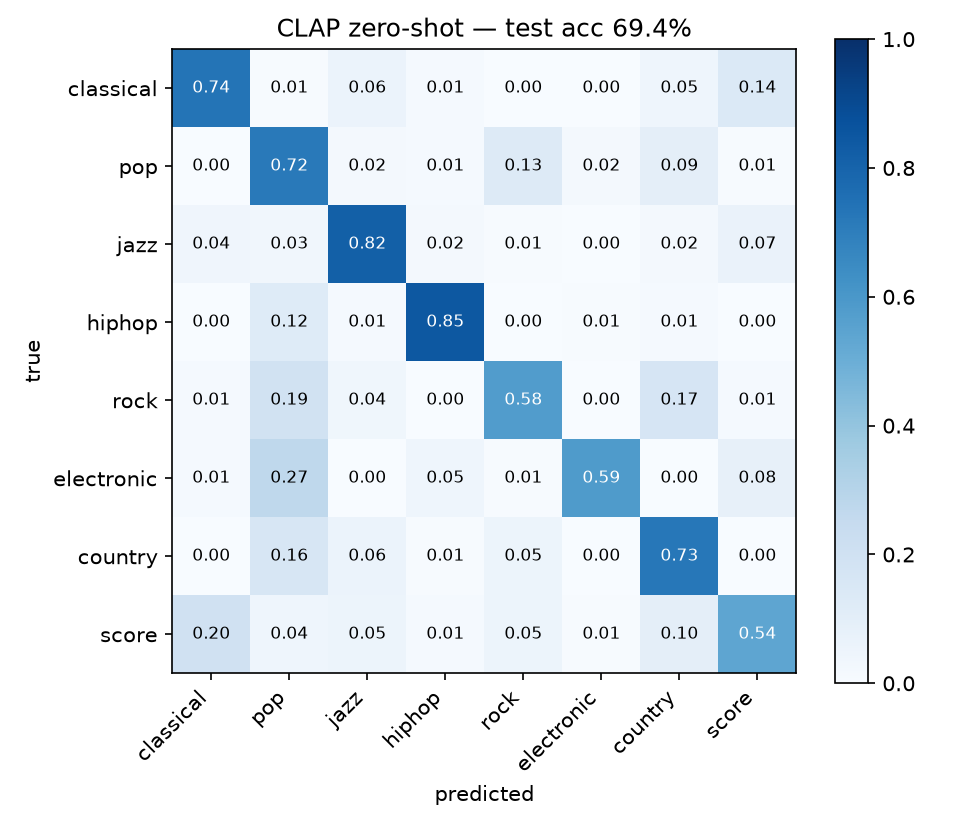
\includegraphics[width=.49\textwidth]{clap_larger_clap_general/confusion_test.png}\hfill
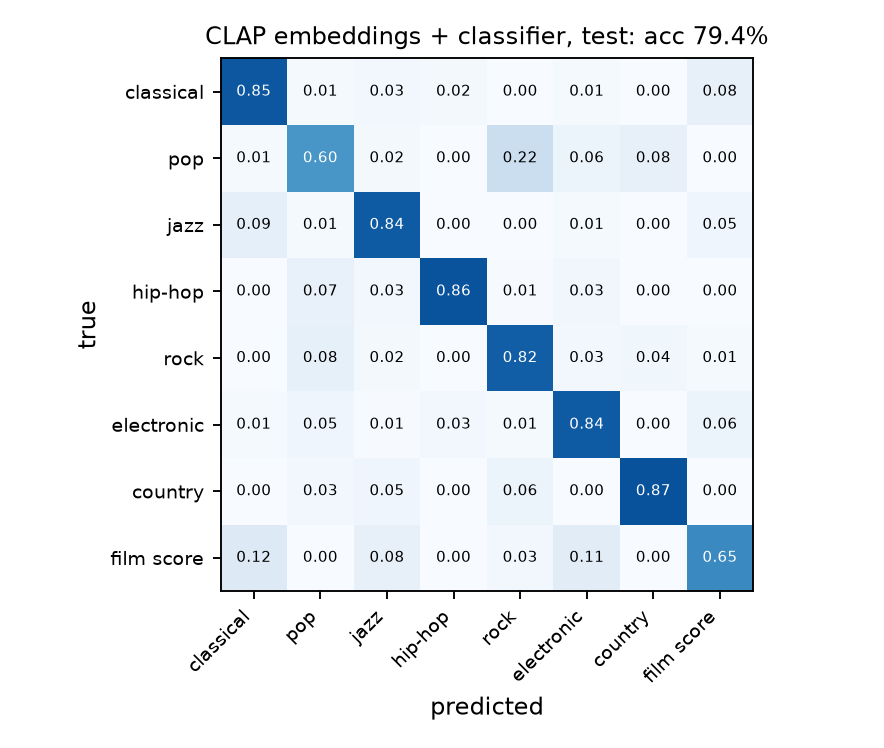
\includegraphics[width=.49\textwidth]{confusion_clap_head_test.png}
\caption{Left: CLAP zero-shot on the test split. Right: the classifier trained on CLAP embeddings. Zero-shot's biggest error is calling electronic music pop.}
\end{figure}
\begin{figure}[H]\centering
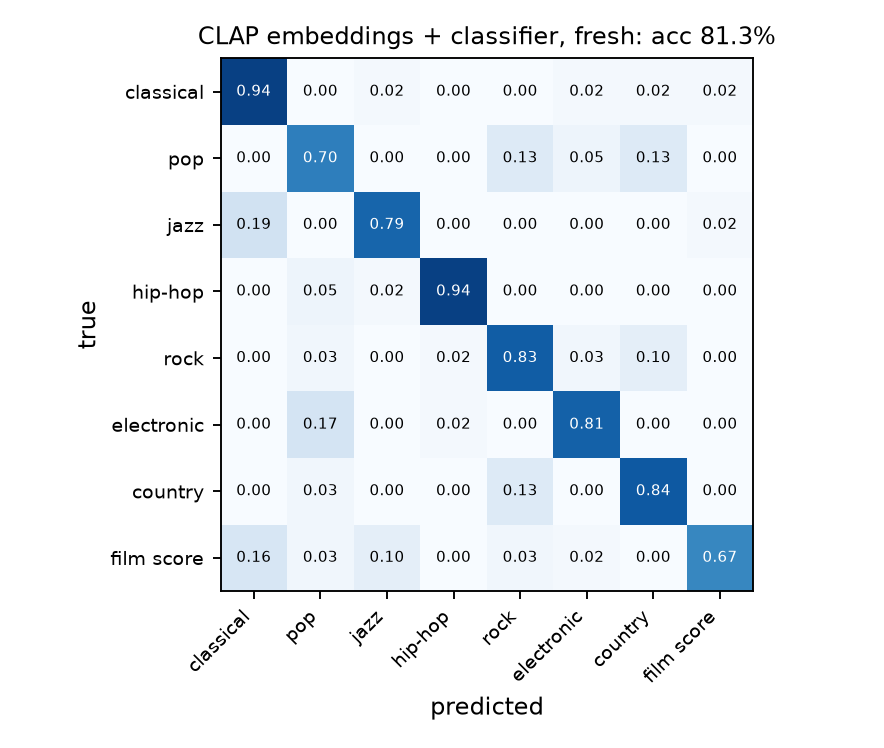
\includegraphics[width=.49\textwidth]{confusion_clap_head_fresh.png}\hfill
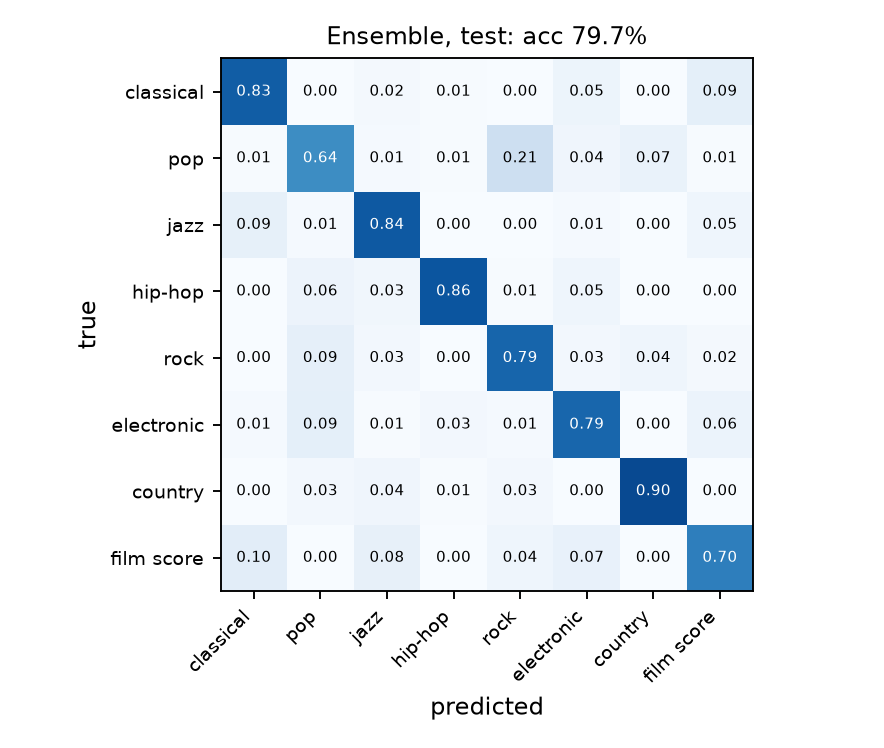
\includegraphics[width=.49\textwidth]{confusion_ensemble_test.png}
\caption{Left: the CLAP classifier on the fresh set. Right: the ensemble on the test split. The ensemble's matrix is almost the CLAP classifier's: the two models agree on 77\,\% of clips.}
\end{figure}
\begin{figure}[H]\centering
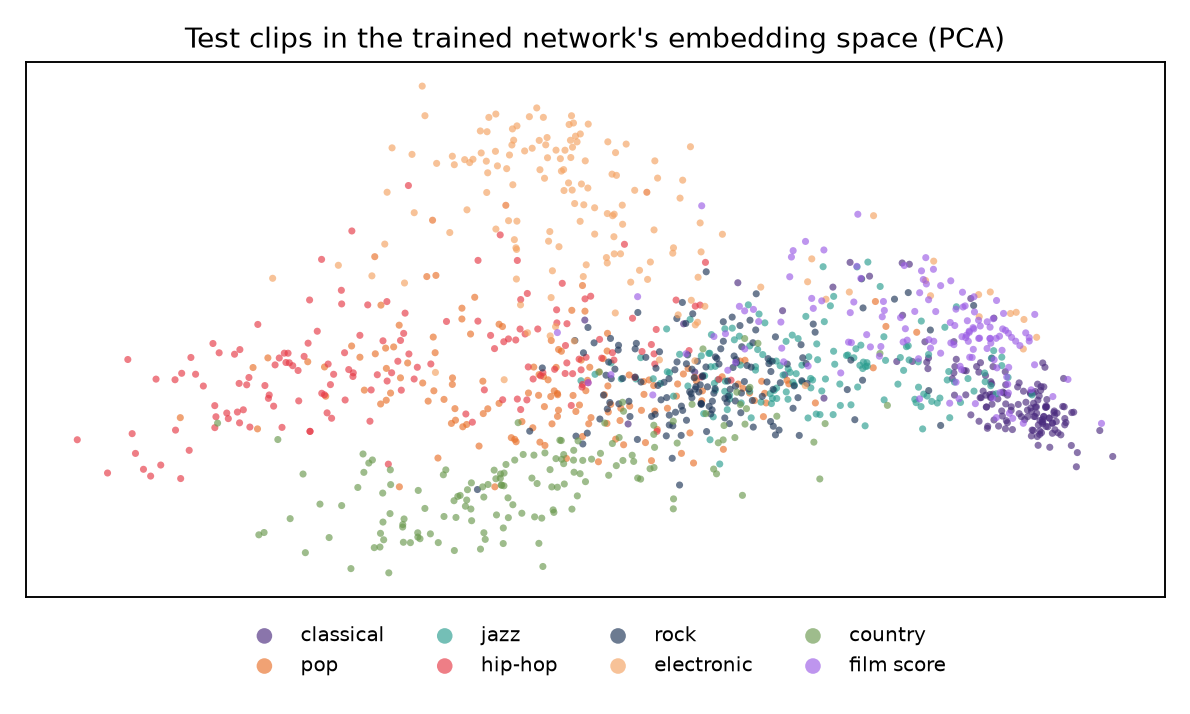
\includegraphics[width=.7\textwidth]{embedding_pca.png}
\caption{The test clips in the CNN's own 512-dimensional embedding space, projected to two dimensions. Classical and film score sit at one end, hip-hop and country at the other, and electronic breaks off on its own. Pop is spread across the middle.}
\end{figure}
Zero-shot CLAP is impressive for zero training but loses to the small CNN on both sets. Its biggest error is calling electronic music pop, 40 of the 63 fresh electronic clips, and its country F1 is twenty points below the CNN's. These are partly prompt problems: ``electronic dance music'' is narrower than Deezer's electronic tag, and I never tuned the wording. The classifier on CLAP embeddings, by contrast, beats every CNN on both sets, by about two points over cnn\_v4 and four over cnn\_v3, with the largest gains on electronic, pop and film score. The CNN holds its own on country and classical.

On the fresh set the two best models agree on 77\,\% of clips. Both are right on 65\,\%, only the CNN on 12\,\%, only the CLAP classifier on 8\,\%, and both wrong on 15\,\%. Those 74 clips are mostly pop, electronic and the classical-versus-score pair: the genuinely ambiguous songs. The ensemble, which averages the two, adds only 0.3 points for the same reason.

\subsection{Does more data help?}
cnn\_v3 and cnn\_v4 differ in two ways, 2.3 times the training clips and 2.2 times the parameters, and together those bought 2.0 points on the test split and 1.6 on the fresh set. Earlier in the project, going from 10\,208 to 11\,238 clips (cnn\_v1 to cnn\_v2) bought one point, almost all of it on classical, the one genre that had been short. In the voice project, going from 4\,000 to 20\,000 clips bought twelve points. So more data helps, and helps most when a class is short, but the slope flattens: a straight-line extrapolation of the music results says 100\,000 clips would reach the low 80s, not 90.

\subsection{The demo}
A small local web page (\texttt{src/app.py}) takes any MP3 of any length, or a song name, and shows the album cover, a ten-second player, the probability for every genre, and the spectrogram with the network's guess written over each five-second window. It can run the CNN and the CLAP classifier side by side, or their ensemble. Some class examples: Beethoven's Moonlight Sonata $\to$ classical 94\,\%; Miles Davis, ``So What'' $\to$ jazz 97\,\%; Kendrick Lamar, ``HUMBLE.'' $\to$ hip-hop 97\,\%; Hans Zimmer, ``Time'' $\to$ film score 90\,\%; Dolly Parton, ``Jolene'' $\to$ country 49\,\% / pop 46\,\% from the CNN but country 96\,\% from CLAP. Watching the guess change every five seconds taught me more about what the model hears than any table.

\section{Discussion and conclusion}\label{sec:discussion}

\subsection{Sound is about mixtures}
Both questions were hardest exactly where things overlap. The voice counter's worst case is three simultaneous speakers; its real-world weakness is two people briefly talking over each other. The genre model's worst cases are pop, which overlaps with everything, and classical against film score, which share an orchestra. A photograph lets a network draw a box around each object. A waveform makes it separate the objects from one signal first. The spectrogram helps, because it spreads sources out in pitch as well as time, but it does not undo the mixing.

\subsection{Data decides}
The clearest result in the project is the fall from 80 to 25\,\% when the voice counter moved from simulated rooms to real ones. The network had learned the simulation, not the task. Nothing about the network changed when it recovered to 68\,\%; only the data did. The music half, built with real data from the start, never had that cliff, but it hit a different wall: its remaining errors live in the labels. Deezer tags whole albums, pop is a catch-all, and film scores are orchestral music. Published studies of human agreement on broad genre labels land around 75 to 85\,\%, which is exactly where every model here landed. In both halves, better data beat a better network, and the biggest single gain of the whole project, twelve points, came from five times more training clips with no change to the model.

\subsection{Borrowed ears beat home-made ones}
A classifier with 130\,000 parameters trained for three minutes on CLAP's embeddings beat a 5.5-million-parameter CNN trained for two hours on twice the data. CLAP already knows what music sounds like, and my labels only had to teach it where my genre boundaries fall. This is the usual story in modern machine learning, and it was useful to see it happen on my own data: when a model exists that has already listened to the world, start from it. The CNN is not useless, it wins on country and is ten times faster at inference, but it is no longer the headline.

\subsection{Honest testing}
Three choices kept the numbers trustworthy. Splitting by speaker and by artist, rather than by clip, forced the models to generalise to new voices and new performers. Freezing the validation and test clips before the second crawl made every model comparable. And the fresh 504 songs, scraped after all the modelling was done, confirmed that nothing had been tuned to the test split: every model scored two to three points higher on them, with the same ranking. One number I report with a caveat is the single-sex experiment, where the splits overlapped slightly.

\subsection{Practical lessons}
Some of the project's hours went to problems that have nothing to do with neural networks, and they are worth recording. Deezer's preview links expire within minutes. Its server throttles after about ten thousand fast downloads. A public model can load without any error and still be broken under a new library version, which I caught only because every prediction came out at exactly 12.5\,\%. And a laptop silently slows its GPU three-fold the moment the charger comes out, which turned a nine-minute epoch into a thirty-minute one twice.

\subsection{Conclusion}
A small CNN on a laptop can count voices in a noisy room to within one person 99\,\% of the time, and name the genre of a song by an unknown artist about four times out of five. Both numbers are set by the data more than by the model. Where a model trained on far more sound exists, a thin layer on top of it is the better starting point. And the mistakes that remain, two voices briefly overlapping, pop against rock, orchestra against film score, are the ones people make too.

\section{Future work: had I had more time}\label{sec:future}
\begin{itemize}
  \item \textbf{Fine-tune CLAP itself.} The classifier on frozen embeddings is a lower bound. Unfreezing the audio encoder and training it end-to-end on my 23\,000 clips is the obvious next step and would probably clear 85\,\%.
  \item \textbf{Tune the zero-shot prompts.} The prompts were my first guess. Choosing them on the validation split would likely move zero-shot from 69\,\% into the low 70s, and it would make a good classroom demonstration of a model's accuracy swinging on word choice alone.
  \item \textbf{Scale the data.} 100\,000 clips is about a day of work: 48\,GB of audio collected at a polite rate, a loader that streams features from disk instead of holding them in memory, and a 10-million-parameter network trained overnight with the charger attached. The learning curve so far says this is worth three to five points, not fifteen.
  \item \textbf{Clean up the labels.} Drop albums whose tag disagrees with the artist's majority genre, or allow two labels per song. Report accuracy with pop excluded to show what the model does on well-defined genres.
  \item \textbf{Give cnn\_v4 the epochs it wanted.} Its validation accuracy was still rising at epoch eleven; the run was cut to fit a four-hour window.
  \item \textbf{Full songs, not previews.} Train and test on whole tracks and average predictions over the song; the clip-length experiment suggests a few points are available.
  \item \textbf{Back to voices with the same trick.} Retrain the voice counter on a mixture of synthetic and real data, and try a pretrained speech model's embeddings the way CLAP was used for music.
  \item \textbf{A proper listening test.} Several listeners on a few hundred clips, for both tasks, to put a real human number next to the models.
\end{itemize}

\section*{Code and files}
Everything lives in \texttt{\textasciitilde/Desktop/College/FYS}.
\begin{itemize}
  \item \texttt{src/}, \texttt{results/}, \texttt{slides/}: the voice-counting project (\texttt{make\_mixtures.py}, \texttt{make\_ami\_windows.py}, \texttt{train.py}, \texttt{evaluate.py}).
  \item \texttt{genre/src/}: \texttt{scrape\_deezer.py}, \texttt{crawl\_score.py}, \texttt{extend\_data.py}, \texttt{preprocess.py}, \texttt{train.py}, \texttt{evaluate.py}, \texttt{clap\_zero.py}, \texttt{clap\_embed.py}, \texttt{clap\_head.py}, \texttt{eval\_all.py}, \texttt{fresh\_test.py}, \texttt{app.py} (the demo).
  \item \texttt{genre/results/comparison.json}: every number in Table~\ref{tab:final}; \texttt{genre/results/dataset/}: the data figures; \texttt{genre/slides/}: the decks.
\end{itemize}
\begin{lstlisting}[language=bash]
python src/scrape_deezer.py && python src/crawl_score.py && python src/preprocess.py
python src/train.py --name cnn_v4_w48 --width 48 --epochs 11
python src/clap_embed.py && python src/clap_head.py
python src/eval_all.py cnn_v4_w48 clap_head "ensemble:cnn_v4_w48+clap_head"
python src/app.py        # http://127.0.0.1:8765
\end{lstlisting}
\end{document}
